\documentclass[a4paper]{article}

\usepackage{graphicx}
\usepackage{listings}
\usepackage{amsmath}

\begin{document}

\title{ELEC5507 Assignment}
\author{Vanush Vaswani - ********* \\
Zhaoyan Liu - 440092733 \\
Stephen Tridgell - 309205867}

\maketitle


\lstset{language=Matlab}

The goal of error control coding is to encode messages for transmission with redundancy such that the receiver can correct the errors in the transmission and recover the original data. In this project, encoders and decoders will be simulated and analysed by using MATLAB. The first section involves the design and simulation of the BCH code over BSC and AWGN channels. The second section uses LDPC codes to meet the requirements of a power limited system with very high reliability. Similar simulations are run and compared with the results of the BCH code.

\section*{Section 1}

\subsubsection*{Question 1} \textit{What is the generator polynomial for this code? Use MATLAB’s ’bchgenpoly’ function to verify your answer} \\
\\
The generator polynomial for a n = 31, k = 16, and t = 3 BCH code is $g(x) = x^{15} + x^{11} + 
x^{10} + x^{9} + x^{8} + x^{7} + x^{5} + x^{3} + x^{2} + x^{1} + 1$. 
This was verified with 
\begin{lstlisting}
[gen, t] = bchgenpoly(31,16)
\end{lstlisting}

\subsubsection*{Question 2} \textit{What is the minimum distance of this code?} \\
\\
For a BCH code, $d_{min} \geq 2*t + 1 = 7$, this was verified using 
\begin{lstlisting}
gfweight(double(gen.x), 31)
\end{lstlisting}
which gave a minimum distance calculation of 7.

\subsubsection*{Question 3} \textit{Construct the reduced syndrome lookup table for this code. You need to write a program to do this since it is difficult to do it by hand. You do not need to include the whole array in your report due to its large size. Instead, just show the sub-array consisting of the first 5 rows in your report, and include a separate text file (*.txt) enumerating all the data in your electronic submission.} \\
\\
Generate the syndrome lookup table by:
\begin{lstlisting}
[h g k] = cyclgen(31, double(gen.x))
trt = syndtable(h)
\end{lstlisting}

The first 5 rows are:\\
\scalebox{0.7}{
\begin{tabular}{| *{31}{c} |}
\hline
0 & 0 & 0 & 0 & 0 & 0 & 0 & 0 & 0 & 0 & 0 & 0 & 0 & 0 & 0 & 0 & 0 & 0 & 0 & 0 & 0 & 0 & 0 & 0 & 0 & 0 & 0 & 0 & 0 & 0 & 0 \\
\hline
0 & 0 & 0 & 0 & 0 & 0 & 0 & 0 & 0 & 0 & 0 & 0 & 0 & 0 & \textbf{1} & 0 & 0 & 0 & 0 & 0 & 0 & 0 & 0 & 0 & 0 & 0 & 0 & 0 & 0 & 0 & 0 \\
\hline
0 & 0 & 0 & 0 & 0 & 0 & 0 & 0 & 0 & 0 & 0 & 0 & 0 & \textbf{1} & 0 & 0 & 0 & 0 & 0 & 0 & 0 & 0 & 0 & 0 & 0 & 0 & 0 & 0 & 0 & 0 & 0 \\
\hline
0 & 0 & 0 & 0 & 0 & 0 & 0 & 0 & 0 & 0 & 0 & 0 & 0 & \textbf{1} & \textbf{1} & 0 & 0 & 0 & 0 & 0 & 0 & 0 & 0 & 0 & 0 & 0 & 0 & 0 & 0 & 0 & 0 \\
\hline
0 & 0 & 0 & 0 & 0 & 0 & 0 & 0 & 0 & 0 & 0 & 0 & \textbf{1} & 0 & 0 & 0 & 0 & 0 & 0 & 0 & 0 & 0 & 0 & 0 & 0 & 0 & 0 & 0 & 0 & 0 & 0 \\
\hline
\end{tabular}
}

The corresponding syndromes for these error patterns are:\\
\begin{tabular}{| *{15}{c} | c c |}
\hline
0 & 0 & 0 & 0 & 0 & 0 & 0 & 0 & 0 & 0 & 0 & 0 & 0 & 0 & 0 & = & \textbf{0}  \\
\hline
0 & 0 & 0 & 0 & 0 & 0 & 0 & 0 & 0 & 0 & 0 & 0 & 0 & 0 & \textbf{1} & = & \textbf{1}  \\
\hline
0 & 0 & 0 & 0 & 0 & 0 & 0 & 0 & 0 & 0 & 0 & 0 & 0 & \textbf{1} & 0 & = & \textbf{2}  \\
\hline
0 & 0 & 0 & 0 & 0 & 0 & 0 & 0 & 0 & 0 & 0 & 0 & 0 & \textbf{1} & \textbf{1} & = & \textbf{3}  \\
\hline
0 & 0 & 0 & 0 & 0 & 0 & 0 & 0 & 0 & 0 & 0 & 0 & \textbf{1} & 0 & 0 & = & \textbf{4}  \\
\hline
\end{tabular}\\
\\
The rest of the array is in "trt.csv".

\subsubsection*{Question 4} \textit{Based on the standard array you obtained in task 3, find out the weight distribution of the coset leaders.}
\begin{lstlisting}
weights = sum(trt')
A0 = sum(weights == 0)
A1 = sum(weights == 1)
A2 = sum(weights == 2)
A3 = sum(weights == 3)
A4 = sum(weights == 4)
A5 = sum(weights == 5)
\end{lstlisting}
Gives the weight distribution of $A_0 = 1$, $A_1 = 31$, $A_2 = 465$, $A_3 = 4495$, $A_4 = 13020$ and $A_5 = 14756$ where $A_i$ is the number of weight $i$ errors.

\subsubsection*{Question 5} \textit{Design and implement an encoder using the generator polynomial for this BCH code.} \\
\\
The encoder with the generator polynomial was implemented using the cyclic properties of the code. The message, $c(X)$, is shifted by $n-k$ and divided by the generator polynomial to get the parity check bits by $b(X) = remainder[\frac{X^{n-k}c(X)}{g(X)}]$. The parity check bits are combined with the message for a systematic code. The function below shows our implementation.

\lstinputlisting[language=Matlab]{../polBCHencoder.m}

\subsubsection*{Question 6a} \textit{Use MATLAB defined functions (eg. the ”decode” function) to decode the BCH code.}\\
\\
This decoder is implemented using MATLAB’s function \textit{decode()}. The matrix \textit{trt} is the syndrome decoding table calculated above using the \textit{syndtable()} function.

\lstinputlisting[language=Matlab]{../matlabBCHdecode.m}

\subsubsection*{Question 6b} \textit{Design and implement a decoder using the syndrome decoding table in Task 3 for the BCH code.}\\
\\
The syndrome can be obtained by multiplying received codeword with the transposed parity-check matrix H. The corresponded error pattern is found by performing a look up in the trt table calculated above. The corrected code is then the codeword plus the error pattern. Our implementation is shown below.

\lstinputlisting[language=Matlab]{../syndLookupDecode.m}

\subsubsection*{Question 6c} \textit{Design and implement a decoder using the Berlekamp’s iterative procedure.}\\
\\
The implementation of berlekamps iterative procedure below used different notation to the textbook specified in \textit{http://www.mathworks.com.au/help/comm/ug/error-detection-and-correction.html} allowing easier implementation of the procedure.

\lstinputlisting[language=Matlab]{../berlekamp_decode.m}

\subsubsection*{Question 7} \textit{Simulate the implemented BCH encoder and decoder (using ANY method in Part 6) using the attached wave file (austinpowers.wav) in a BSC channel for different transition probabilities. Discuss the impact of changing different transition probability values.}\\
\\
The channel was simulated using the following function:

\lstinputlisting[language=Matlab]{../playAudioOverBSC.m}

Different transition probabilities were input into the function. With a transition probability of below 0.05 the sound could be heard with a little noise audible. As p increased above 0.15 the noise increased to the level where it could no longer be clearly heard. Above 0.2 it was difficult to hear anything at all other than noise.

\subsubsection*{Question 8a and 8b} \textit{Simulation over BSC Simulate the BCH code in a BSC channel (you are allowed to use MATLAB defined functions) and plot the BER versus transition probability for coded and uncoded systems on the same graph. Plot BER versus $\frac{E_b}{N_0}$ for coded and uncoded systems on the same graph by assuming that the SNR ($ = \frac{E_b}{N_0}$ ) is related to the transition probability for the coded system via $X_{dB,coded} = 10 \log_{10}(\frac{[Q^{- 1} (p)]^2}{R}) $ and that for uncoded system is $X_{dB,uncoded} = 20\log_{10}(Q^{- 1} (p)) $, where $Q(x) = \frac{1}{\sqrt{2 \pi}} \int\limits_{x}\limits^{+\infty} e^{ -\frac{z^2}{2}} dz $ and $0 < p < 0.5$.}\\
\textit{Simulation over AWGN channel with BPSK modulation $\{−1, 1\}$ Simulate the BCH code in an AWGN channel (you are allowed to use MATLAB defined functions) and plot the BER versus the signal to noise ratio (SNR) for a BPSK coded and uncoded systems on the same graph by using a hard-decision demodulator and binary decoder.}\\
\\
\lstinputlisting[language=Matlab]{../bch_ber_simulation.m}

This produced the following plots. \\
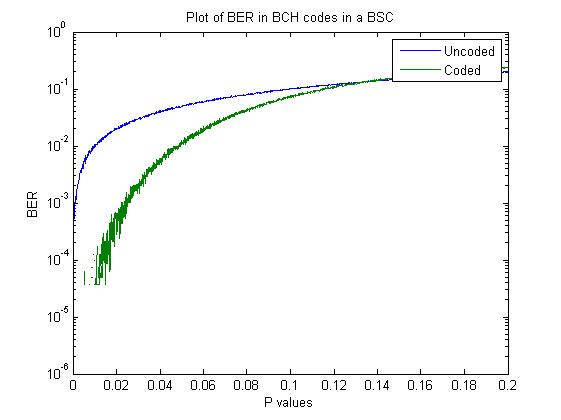
\includegraphics[scale=0.5]{plotBER_BSC_pvals.jpg} \\
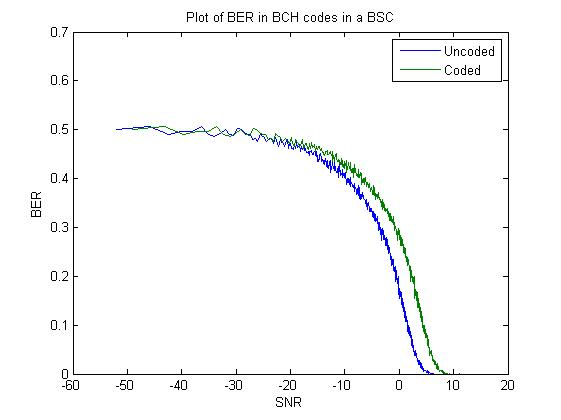
\includegraphics[scale=0.5]{plotBER_BSC_SNR.jpg} \\
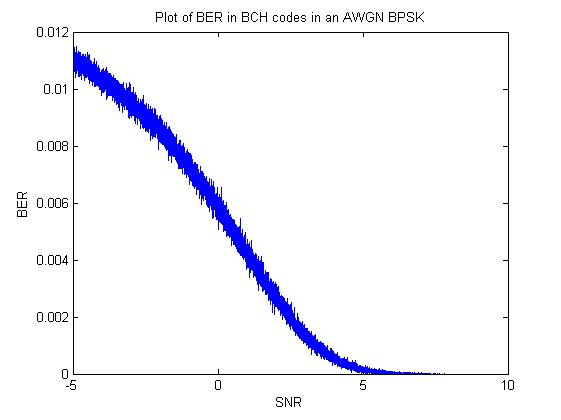
\includegraphics[scale=0.5]{plotBER_AWGN.jpg} \\
\textbf{TODO: RESAVE AWGN plot} 

\subsubsection*{Question 8c} \textit{Draw a table detailing the coding gain for BER$= [10^{−2}, 10^{−3}, 10^{−4} , 10^{−5} , 10^{−6} ]$ by reading the differences between the BER curves for BPSK coded and uncoded systems which have been obtained from simulations in part (a) and (b).} \\
\\
\begin{tabular}{| c | c | c |}
\hline
BER & Coding Gain (Hard decision) & Coding Gain (BSC) \\
\hline
$10^{-2}$ & & \\
\hline
$10^{-3}$ & & \\
\hline
$10^{-4}$ & & \\
\hline
$10^{-5}$ & & \\
\hline
$10^{-6}$ & & \\
\hline
\end{tabular}

\subsubsection*{Question 8d} \textit{Find the asymptotic coding gain when $\frac{Eb}{N0}$ is very large from the formula which is given in the lecture notes and compare with simulation results.} \\
\\
Using the formula $G = 10\log(R(t+1))$ in lecture 5 for large $\frac{Eb}{N0}$ where $R = 16/31$ and $t = 3$ results in a coding gain of $G = 3.1482$ dB. Comparing this to the simulation results \textbf{...} \\

\section*{Section 2}

\textit{You are an engineer whose job is to design and analyze the performance of error control codes for different clients. Client 2 requires a code for satellite transmission of digital TV. The satellite is power limited and very high reliability is required (as close to Shannon capacity as possible). Low decoding complexity is desired, but is not essential. To meet these requirements an LDPC code is used} \\
\\
\subsubsection*{Question 1} \textit{Design the code (e.g. type of code, code parameters, and other relevant information) and justify its design}\\
\\
Answer here \\

\subsubsection*{Question 2} \textit{Simulate the chosen code using the attached wave file (austinpowers.wav) in a BSC channel for different transition probabilities (you are allowed to use MATLAB defined functions. Discuss the difference in sound quality compared to the BCH code in Section I, for different transition probabilities.}\\
\\
Answer here \\

\subsubsection*{Question 3a}\textit{Simulate the chosen code in a BSC channel (you are allowed to use MATLAB defined functions) and plot the BER versus transition probability for coded and uncoded systems on the same graph. Plot BER versus $\frac{E_b}{N_0}$ for coded and uncoded systems on the same graph by assuming that the SNR ($ = \frac{E_b}{N_0}$ ) is related to the transition probability for the coded system via $X_{dB,coded} = 10 \log_{10}(\frac{[Q^{−1} (p)]^2}{R}) $ and that for uncoded system is $X_{dB,uncoded} = 20\log_{10}(Q^{−1} (p)) $, where $Q(x) = \frac{1}{\sqrt{2 \pi}} \int\limits_{x}\limits^{+\infty} e^{ -\frac{z^2}{2}} dz $ and $0 < p < 0.5$.} \\
\\
Answer here \\

\subsubsection*{Question 3b} \textit{Simulate the chosen code in an AWGN channel (you are allowed to use MATLAB defined functions) and plot the BER versus the signal to noise ratio (SNR) for a BPSK coded and uncoded systems on the same graph by using a hard-decision demodulator and binary decoder. Simulate the chosen code in an AWGN channel and plot the BER versus SNR on the same graph for a BPSK coded system by using a soft-decision decoder.} \\
\\
Answer here \\

\subsubsection*{Question 3c} \textit{Draw a table detailing the coding gain for BER$= [10^{−2}, 10^{−3}, 10^{−4} , 10^{−5} , 10^{−6} ]$ by reading the differences between the BER curves for BPSK coded and uncoded systems which have been obtained from simulations in part (a) and (b).}\\
\\
\begin{tabular}{| c | c | c |}
\hline
BER & Coding Gain (Hard decision) & Coding Gain (BSC) \\
\hline
$10^{-2}$ & & \\
\hline
$10^{-3}$ & & \\
\hline
$10^{-4}$ & & \\
\hline
$10^{-5}$ & & \\
\hline
$10^{-6}$ & & \\
\hline
\end{tabular}

\subsubsection*{Question 3d} \textit{Find the asymptotic coding gain when $\frac{Eb}{N0}$ is very large from the formula which is given in the lecture notes and compare with simulation results.} \\
\\
Answer here \\

\subsubsection*{Question 4} \textit{Discuss the advantages/disadvantages of the code chosen in this section with the BCH code in Section 1 (eg. complexity, coding gain, efficiency)}\\
\\
Answer here \\

\end{document}